\chapter{Introduction}\label{ch:introduction}
In this chapter, the project is introduced and motivated. Furthermore, a brief description is presented for stereo vision and the use for it at HSA Systems, the company with whom the work has been conducted. Lastly, this chapter also describes a delimitation of the project and report.\\

\section{Introduction to stereo vision}\label{sec:stereo vision}
\begin{figure}[ht!]
  \centering
  \begin{subfigure}[t]{0.45\textwidth}
    \centering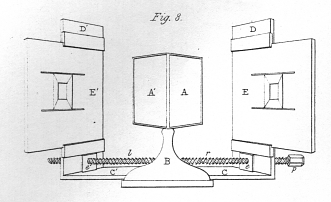
\includegraphics[height=4cm]{figures/paper1-fig08}
    \caption{Wheatstones stereoscope seen from the front\label{fig:wheatstef}}
  \end{subfigure}\hspace{0.5cm}
  \begin{subfigure}[t]{0.45\textwidth}
    \centering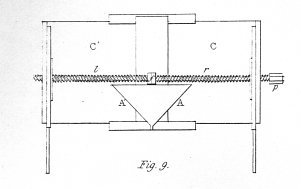
\includegraphics[height=4cm]{figures/paper1-fig09}
    \caption{Wheatstones stereoscope seen from above\label{fig:wheatstet}}
  \end{subfigure}
  \caption{Illustration of Wheatstone's stereoscope from \cite{wheatstone1838contributions}\label{fig:wheatsteall}}
\end{figure}
In 280 A.D the greek mathematician Euclid discovered that the perception of depth is caused by each eye receiving a dissimilar image of the same object. Throughout history, different people have been working on this concept. In 1833 Sir Charles Wheatstone began to mimic depth perception and forced the perception of depth by developing the stereoscope and his work on this is discussed in \cite{wheatstone1838contributions}. Figure \vref{fig:wheatsteall} shows some illustrations of Wheatstones stereoscope. This stereoscope functions by using either two drawings or photographs where the point of view is displaced horizontally by a short distance. These images are placed on the two surfaces marked E' and E on figure \vref{fig:wheatstef}. A' and A on the same figure is two mirrors angled at 45$^{\circ}$ which reflect the images to the viewer. When the viewer move close enough to the mirrors A' and A then the images will be isolated to each eye. This mimics the normal human depth perception and should trigger the brain to accept the images as a single 3D image. \cite{lit:historyofstereophoto}\\

Around 1970, computer vision began appearing and a significant part of this research area is focused on stereo vision: the measurement of depth mimicking the human vision using two cameras \cite{Szeliski2010}. The ability to measure depth enables a computer to distinguish between objects and hence to better interact with and react to the world. This project adds to this research by discussing various aspects of obtaining real time execution without neglecting the quality of the stereo matching.\\

\section{HSA Systems}
\begin{figure}[ht!]
  \centering
  \begin{subfigure}[t]{0.45\textwidth}
    \centering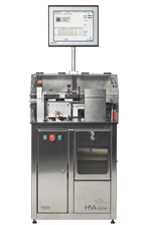
\includegraphics[height=5cm]{figures/pv650_225px}
    \caption{PV650C\cite{HSAsystems}}
    \label{fig:pv650c}
  \end{subfigure}\hspace{0.5cm}
  \begin{subfigure}[t]{0.45\textwidth}
    \centering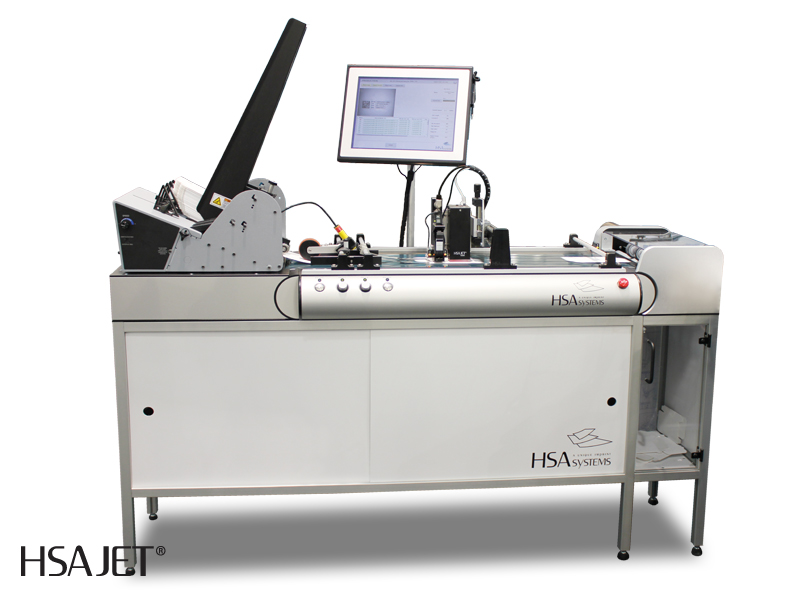
\includegraphics[height=5cm]{figures/layflat1_big}
    \caption{Pharma lay-flat media \cite{HSAsystems}\label{fig:layflat}}
  \end{subfigure}
  \caption{Some products from HSA Systems \label{fig:hsasproducts}}
\end{figure}
HSA Systems is a danish company with an R\&D department in Aalborg, which develops and manufactures high-resolution inkjet printer systems and a range of other products. Figure \vref{fig:hsasproducts} shows two examples of these printer systems. These systems print labels, bar codes etc. on packages and verify the quality print.\\

HSA Systems wishes to track packages going through their printer systems. A strategically placed stereo vision camera will provide knowledge of how many and where these packages are in the printer system. In case of errors and the like, the printer system is then able to notice when the conveyor belt in their system is empty and ready to reset. This is a significant improvement to the current solution at HSA Systems where no knowledge of locations of packages is available except for a single camera scanning labels. Currently in case of errors the conveyor belt is set to run for a set time until it is assumed that the belt is empty.\\

Currently some products exist which can produce real time depth images such as the Asus Xtion PRO \cite{asusxtion} but these 3D sensors have a low depth resolution due to using small image resolution i.e. VGA ($640\times 480$).\\

For detecting packages a high depth precision is not needed since packages normally are larger boxes (above $2\times 2\times 2$ \si{\centi\meter}) but HSA Systems would like to develop a stereo vision camera which also can be used for future assignments where depth precision requirement is higher. Hence HSA Systems have given the requirement for the stereo vision system to have very precise depth measurements of \SI{\leq 5}{\milli\meter} at distances between 0.5-1.5 m \label{req:dispre}.

\section{Motivation}\label{sec:intromotiv}
The area of stereo vision has been researched thoroughly and accurate algorithms have been developed but most algorithms are very computationally complex. Some real time algorithms have been developed but these focus on low resolution images. As described HSA Systems wishes for a stereo vision system which can execute in real-time (10 fps) for current assignments \label{req:framerate} while also having a high depth precision for the future assignments. 

\section{Problem description}
As mentioned earlier HSA Systems wishes for stereo vision system which can track packages  going through their printing systems and for future assignments. This project will attempt to develop a stereo vision system which can execute real time and have a high depth precision. This system should be implemented on an FPGA.\\
It is therefore essential that the following questions are asked, and in part we will try to answer them:
\begin{itemize}
  \item What obstacles occur within stereo vision?
  \item Which stereo vision algorithms exist, both being computationally efficient and at the same time providing good vision results?
  \item How can an architecture be designed and optimized for executing a stereo vision algorithm?
\end{itemize}

\section{Delimitation}
This project is mainly concerned with the design and implementation of a hardware architecture on an FPGA. Therefore, we will not focus on developing a new stereo vision algorithm. Limitations and issues with stereo vision algorithms will be analyzed but a simpler solution will be used for most obstacles.

\section{Report Structure and Design Process}\label{sec:a3model}
The A$^3$ model is a basic design model originally suggested by teaching staff at AAU and is illustrated on figure \vref{fig:A3model}. The model consists of three design domains which can be explored and the report is structured after this model. These domains are Application, Algorithm, and Architecture.\\
\begin{figure}[ht!]
  \centering
  \includegraphics[scale=0.25]{figures/A3model.jpg}
  \caption{A$^3$ model}
  \label{fig:A3model}
\end{figure}

The search for a solution starts in the application domain where the problem, the application and the specifications are explored. Chapter \vref{ch:appanalysis}: Application Analysis will explore the Application domain and the resulting specification for the application are presented in chapter \vref{ch:req}. The problem and application - which has been specified by HSA Systems - is specified in this chapter and will be explored further in chapter \vref{ch:appanalysis}.\\

As represented by the solid arrows on figure \vref{fig:A3model}, there are several possible algorithms that may match a specific application and  specification. Similarly, several architectures may be used to implement a given algorithm. Exploration of the algorithm is described in chapter \vref{ch:alganalysis} .\\

Chapter \vref{ch:designmet} will describe a methodology to traverse from an algorithm in the algorithm domain to some hardware architecture in the architecture domain.\\

Notice the dashed arrows in figure \vref{fig:A3model}. These arrows show that when exploring one domain new information might arise which calls for changes in a former domain, and requiring a new iteration through the domains. This basically illustrates that the design process is iterative and thus typically requires several synthesis/evaluation loops before a satisfactory solution is found. In this context "satisfactory" means either compliance with the specification or "best possible".\\

Chapter \vref{ch:acctest} specifies how the testing is done to determine whether the found solution complies with the requirements in chapter \vref{ch:req}. Chapter \vref{ch:conclusion} concludes the project and its findings. 